\begin{figure}[p]
\centering
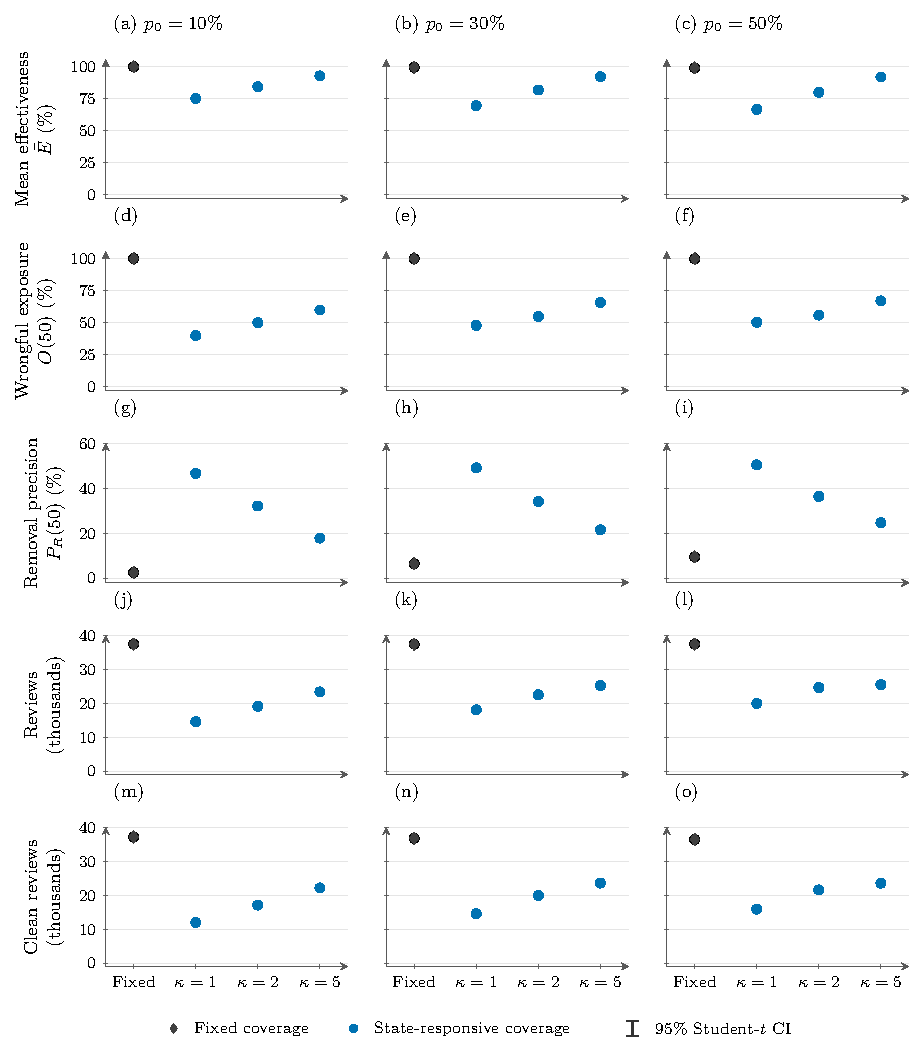
\includegraphics[width=\textwidth,height=0.78\textheight,keepaspectratio]{figures/figS1_workload.pdf}
\caption{Platform workload specifications (P3). Fixed auditing reviews 75\% of accounts per step; responsive auditing uses $\min\{N,\operatorname{round}(0.75N),\operatorname{round}(\kappa I_t)\}$, where $I_t$ is the number of polluted accounts before review and $\kappa=1,2,5$. Both modes use TPR$=$TNR$=80\%$. Points and whiskers show means and 95\% Student-$t$ CIs. Precision is defined in all 30 runs per condition; review counts are in thousands.}
\label{fig:supp-figS1_workload}
\addcontentsline{toc}{subsection}{\protect\numberline{Fig.~\thefigure}Fixed and state-responsive platform auditing}
\end{figure}
\clearpage

\begin{figure}[p]
\centering
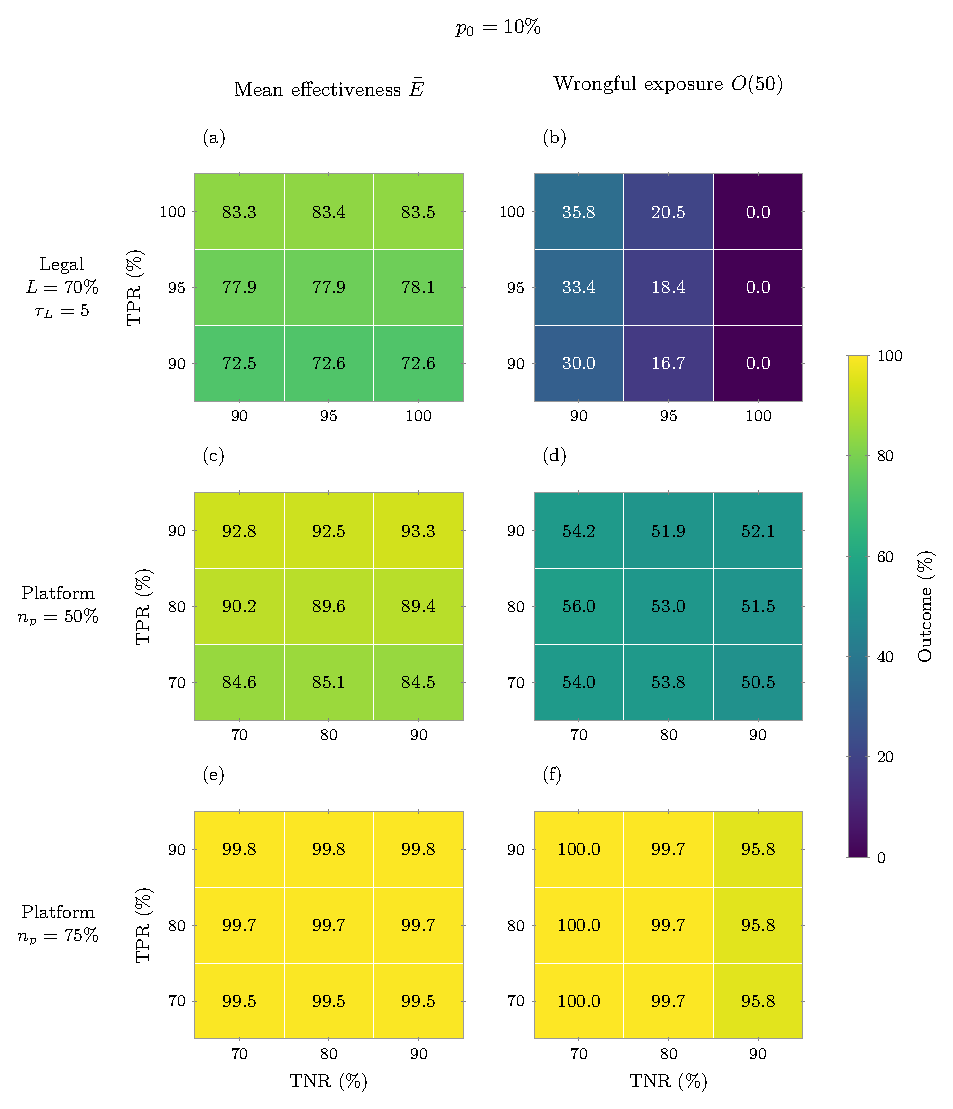
\includegraphics[width=\textwidth,height=0.78\textheight,keepaspectratio]{figures/figS4_accuracy_p10.pdf}
\caption{Independent TPR and TNR variation (P6), $p_0=10\%$. Rows identify governance and coverage settings; platform auditing is fixed. Cells show 30-run means, rounded to one decimal, on a common 0--100\% scale. Full means and 95\% Student-$t$ CIs are retained in the plot CSVs. False-positive flags accumulate wrongful exposure without deleting accounts or links or feeding back into diffusion.}
\label{fig:supp-figS4_accuracy_p10}
\addcontentsline{toc}{subsection}{\protect\numberline{Fig.~\thefigure}Independent TPR/TNR variation: \texorpdfstring{$p_0=10\%$}{p0=10\%}}
\end{figure}
\clearpage

\begin{figure}[p]
\centering
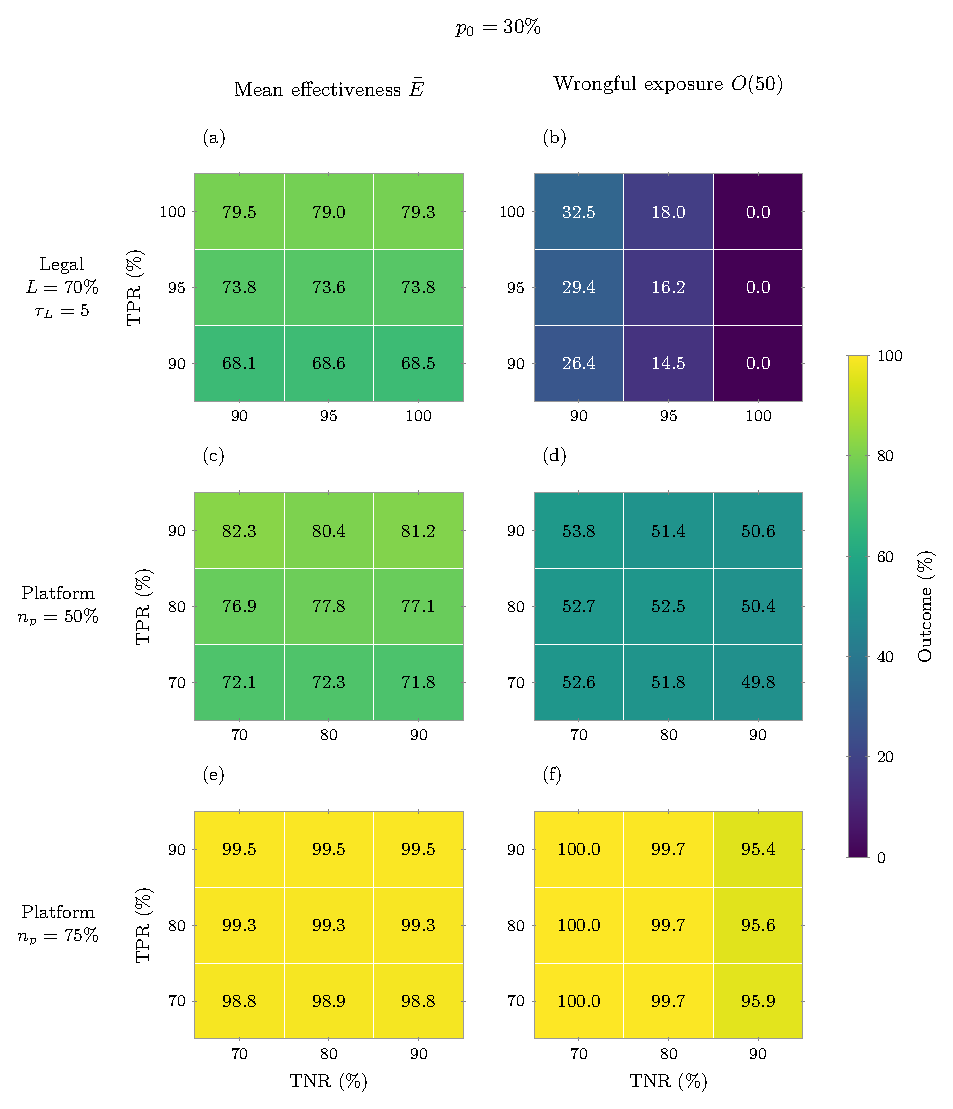
\includegraphics[width=\textwidth,height=0.78\textheight,keepaspectratio]{figures/figS4_accuracy_p30.pdf}
\caption{Independent TPR and TNR variation at $p_0=30\%$. Design, cell summaries and colour scale follow Fig.~\ref{fig:supp-figS4_accuracy_p10}.}
\label{fig:supp-figS4_accuracy_p30}
\addcontentsline{toc}{subsection}{\protect\numberline{Fig.~\thefigure}Independent TPR/TNR variation: \texorpdfstring{$p_0=30\%$}{p0=30\%}}
\end{figure}
\clearpage

\begin{figure}[p]
\centering
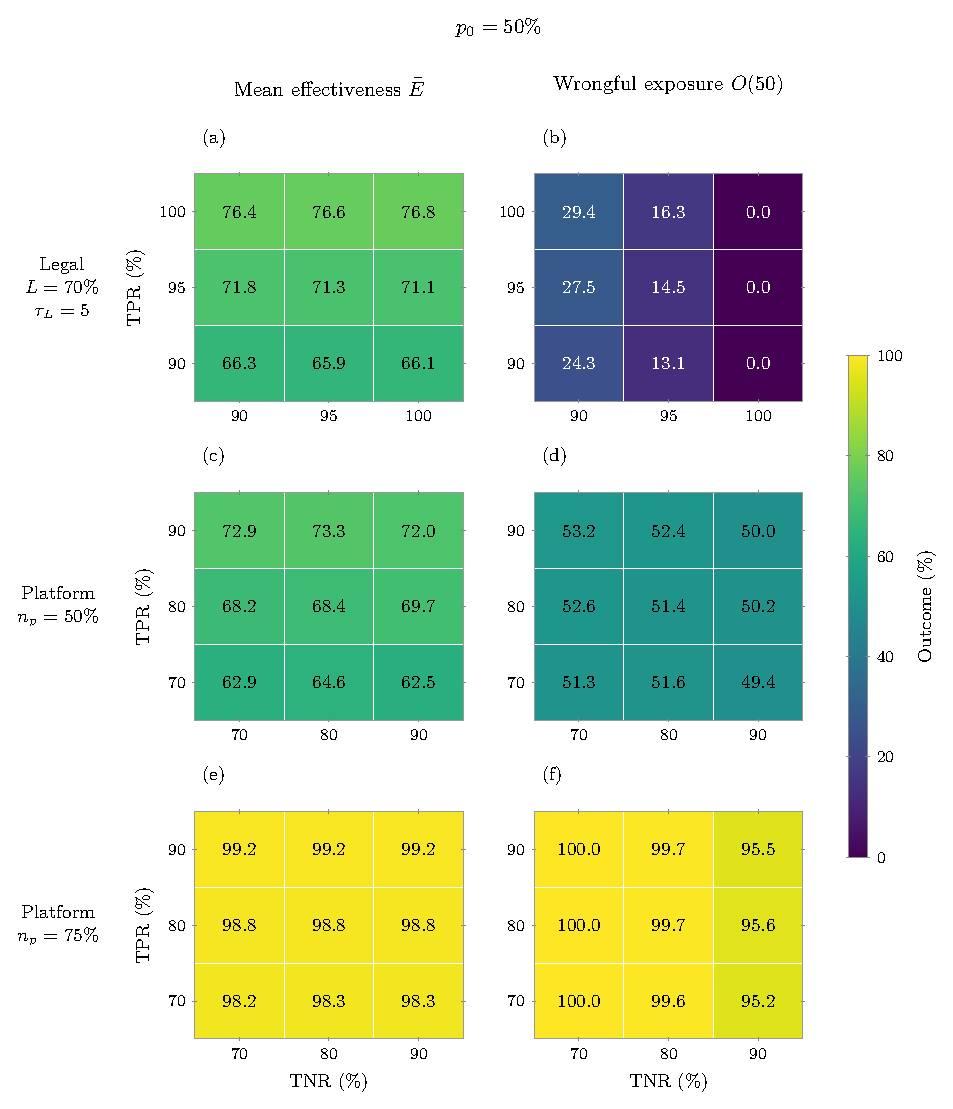
\includegraphics[width=\textwidth,height=0.78\textheight,keepaspectratio]{figures/figS4_accuracy_p50.pdf}
\caption{Independent TPR and TNR variation at $p_0=50\%$. Design, cell summaries and colour scale follow Fig.~\ref{fig:supp-figS4_accuracy_p10}.}
\label{fig:supp-figS4_accuracy_p50}
\addcontentsline{toc}{subsection}{\protect\numberline{Fig.~\thefigure}Independent TPR/TNR variation: \texorpdfstring{$p_0=50\%$}{p0=50\%}}
\end{figure}
\clearpage

\begin{figure}[p]
\centering
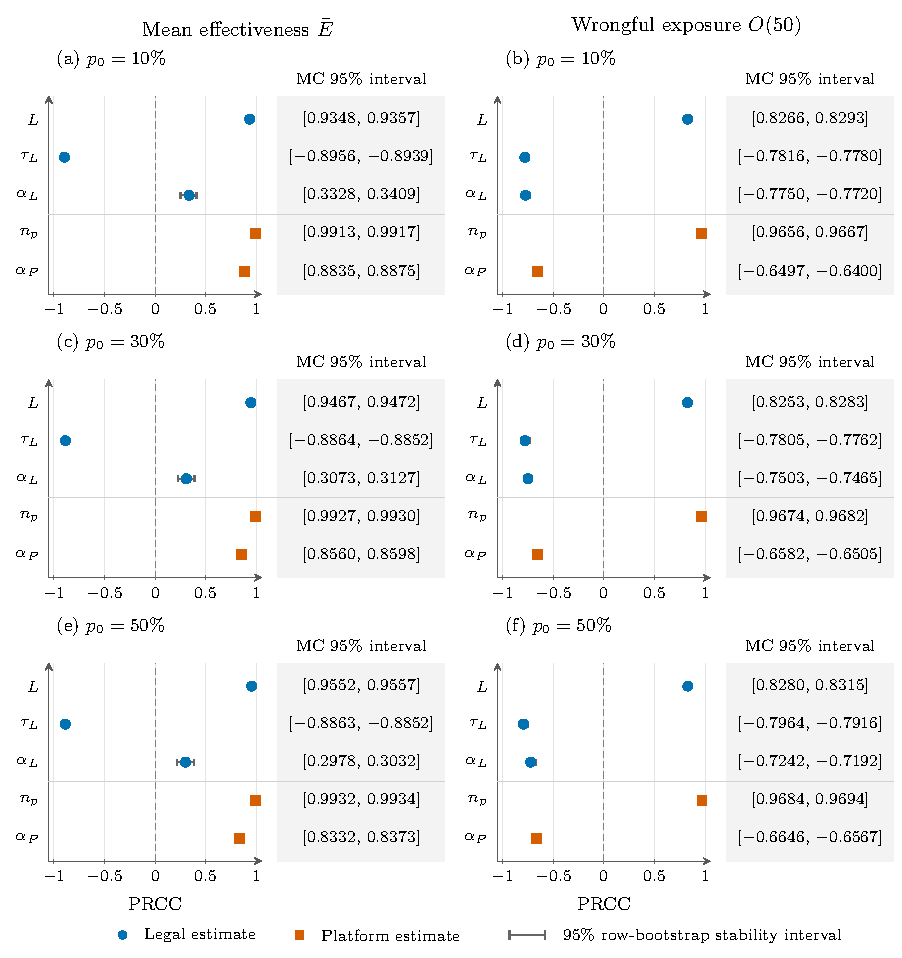
\includegraphics[width=\textwidth,height=0.78\textheight,keepaspectratio]{figures/figS2b_PRCC.pdf}
\caption{Partial rank correlations (PRCC). Points and whiskers show estimates and marginal 95\% row-bootstrap stability intervals; shaded columns report separate 95\% within-point Monte Carlo intervals. Each bootstrap uses 1,000 resamples. Row resampling does not preserve LHS strata. PRCC describes conditional rank association; directional interpretation relies on monotonicity and does not replace the primary PAWN analysis.}
\label{fig:supp-figS2b_PRCC}
\addcontentsline{toc}{subsection}{\protect\numberline{Fig.~\thefigure}PRCC estimates and uncertainty intervals}
\end{figure}
\clearpage

\begin{figure}[p]
\centering
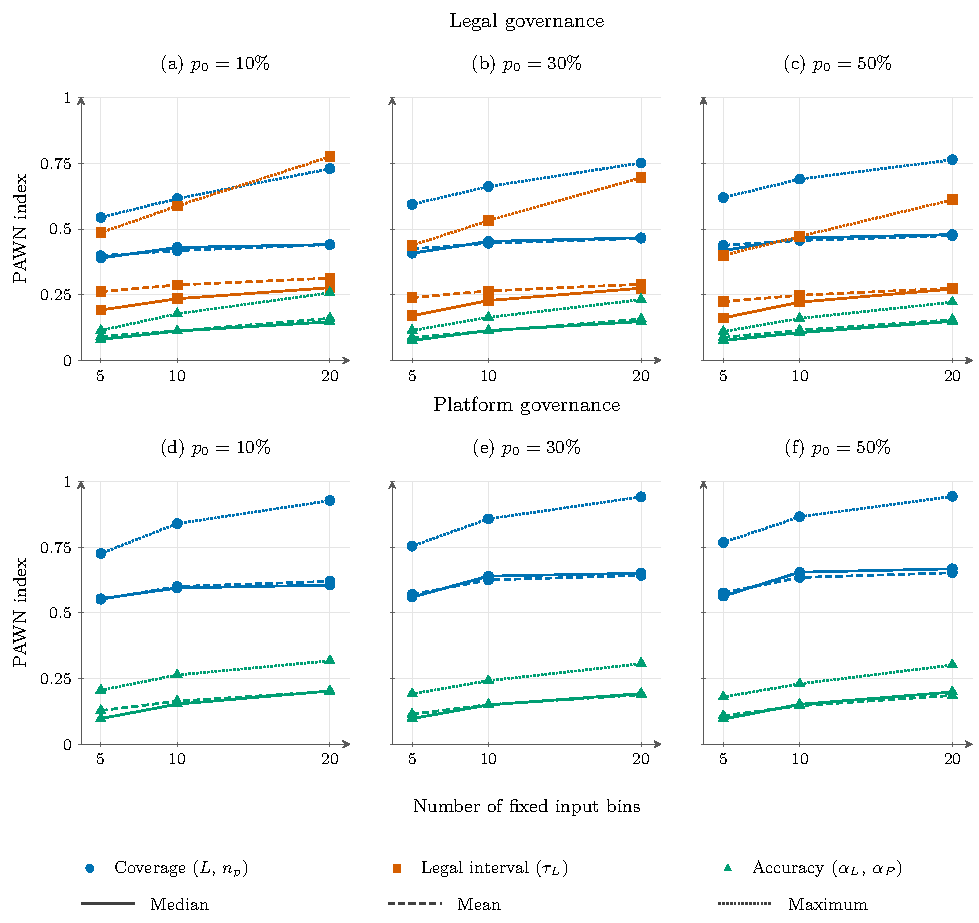
\includegraphics[width=\textwidth,height=0.78\textheight,keepaspectratio]{figures/figS2d_bins_E_mean.pdf}
\caption{PAWN diagnostics for mean effectiveness $\bar E$. Point estimates compare 5, 10 and 20 fixed input bins with median, mean and maximum aggregation; the primary estimator remains the 10-bin median. Full bootstrap intervals, 20- versus 30-run estimates and rankings are provided in \texttt{sensitivity\_diagnostics.csv}.}
\label{fig:supp-figS2d_bins_E_mean}
\addcontentsline{toc}{subsection}{\protect\numberline{Fig.~\thefigure}PAWN diagnostics: mean effectiveness}
\end{figure}
\clearpage

\begin{figure}[p]
\centering
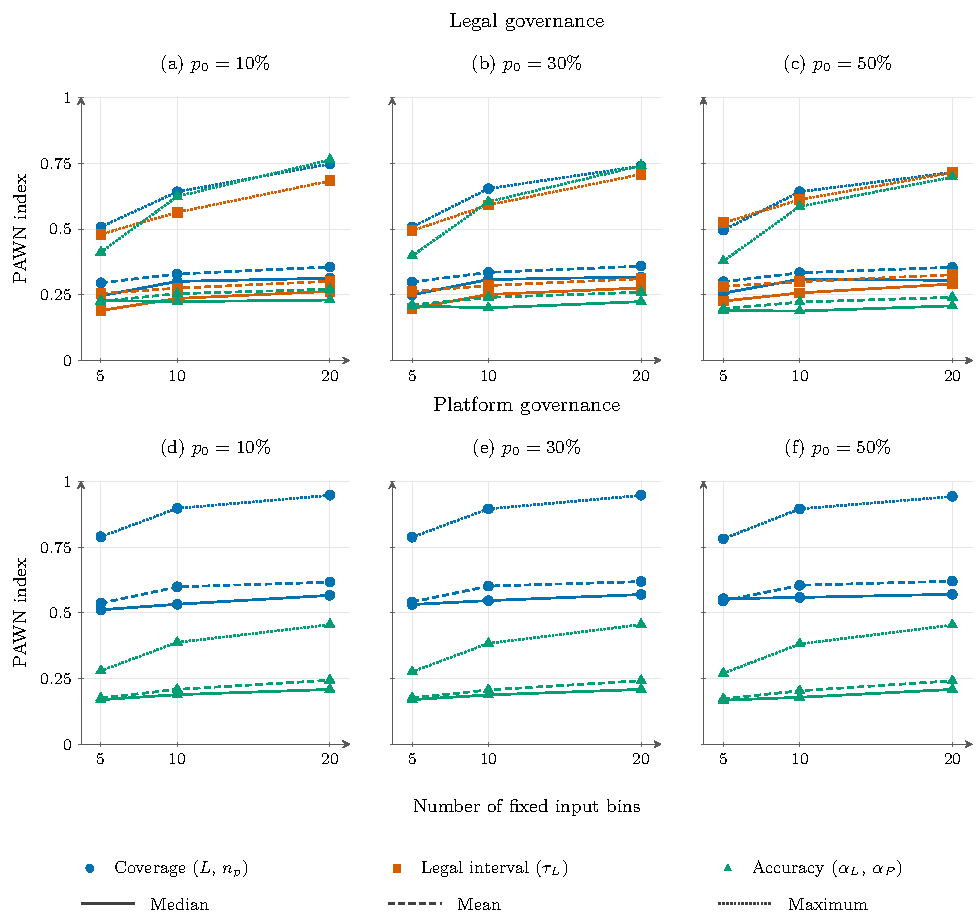
\includegraphics[width=\textwidth,height=0.78\textheight,keepaspectratio]{figures/figS2d_bins_O_final.pdf}
\caption{PAWN diagnostics for wrongful exposure $O(50)$. Settings and graphical encodings follow Fig.~\ref{fig:supp-figS2d_bins_E_mean}.}
\label{fig:supp-figS2d_bins_O_final}
\addcontentsline{toc}{subsection}{\protect\numberline{Fig.~\thefigure}PAWN diagnostics: wrongful exposure}
\end{figure}
\clearpage

\begin{figure}[p]
\centering
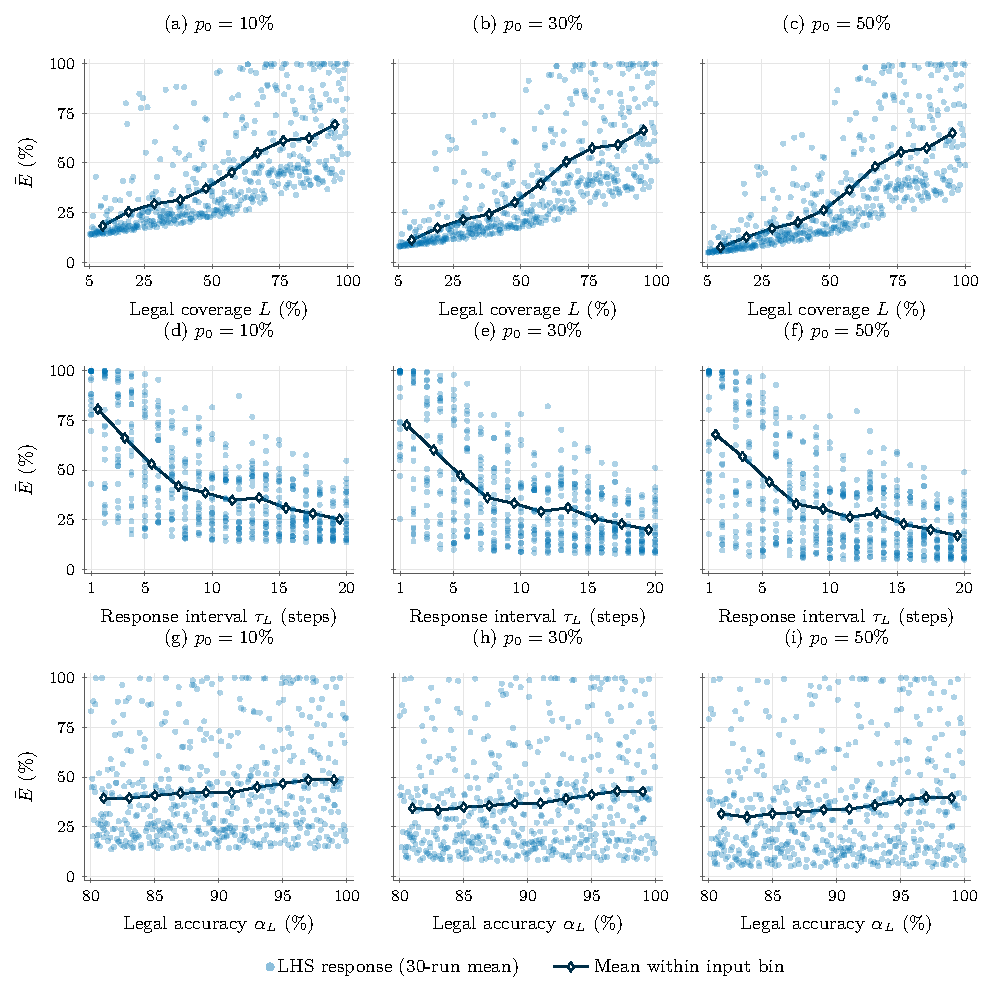
\includegraphics[width=\textwidth,height=0.78\textheight,keepaspectratio]{figures/sensitivity_response_legal_E_mean.pdf}
\caption{Input--response patterns for legal governance and mean effectiveness $\bar E$. Each panel shows 500 LHS responses, each averaged over 30 runs; other inputs vary simultaneously. Lines connect means within 10 fixed input bins. These descriptive summaries are neither isolated single-input causal curves nor confidence bands; they help assess saturation, discreteness and monotonicity.}
\label{fig:supp-sensitivity_response_legal_E_mean}
\addcontentsline{toc}{subsection}{\protect\numberline{Fig.~\thefigure}Legal input--response patterns: mean effectiveness}
\end{figure}
\clearpage

\begin{figure}[p]
\centering
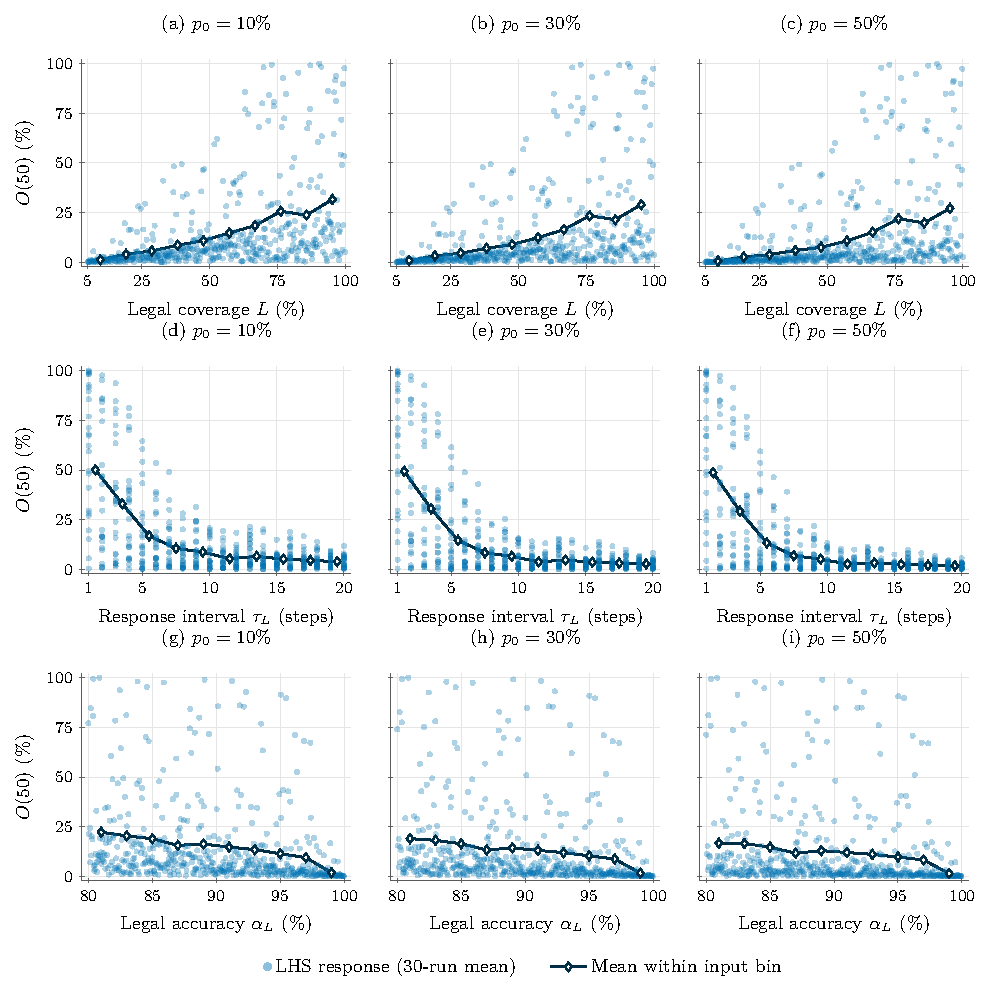
\includegraphics[width=\textwidth,height=0.78\textheight,keepaspectratio]{figures/sensitivity_response_legal_O_final.pdf}
\caption{Input--response patterns for legal governance and wrongful exposure $O(50)$. Sampling, bin summaries and interpretation follow Fig.~\ref{fig:supp-sensitivity_response_legal_E_mean}.}
\label{fig:supp-sensitivity_response_legal_O_final}
\addcontentsline{toc}{subsection}{\protect\numberline{Fig.~\thefigure}Legal input--response patterns: wrongful exposure}
\end{figure}
\clearpage

\begin{figure}[p]
\centering
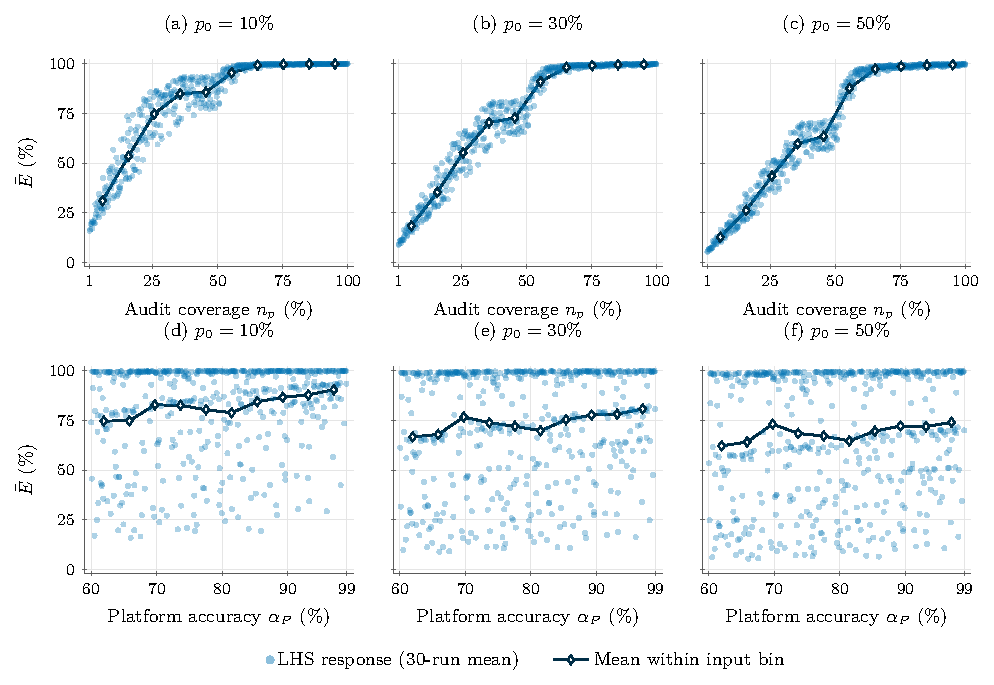
\includegraphics[width=\textwidth,height=0.78\textheight,keepaspectratio]{figures/sensitivity_response_platform_E_mean.pdf}
\caption{Input--response patterns for platform governance and mean effectiveness $\bar E$. Sampling, bin summaries and interpretation follow Fig.~\ref{fig:supp-sensitivity_response_legal_E_mean}.}
\label{fig:supp-sensitivity_response_platform_E_mean}
\addcontentsline{toc}{subsection}{\protect\numberline{Fig.~\thefigure}Platform input--response patterns: mean effectiveness}
\end{figure}
\clearpage

\begin{figure}[p]
\centering
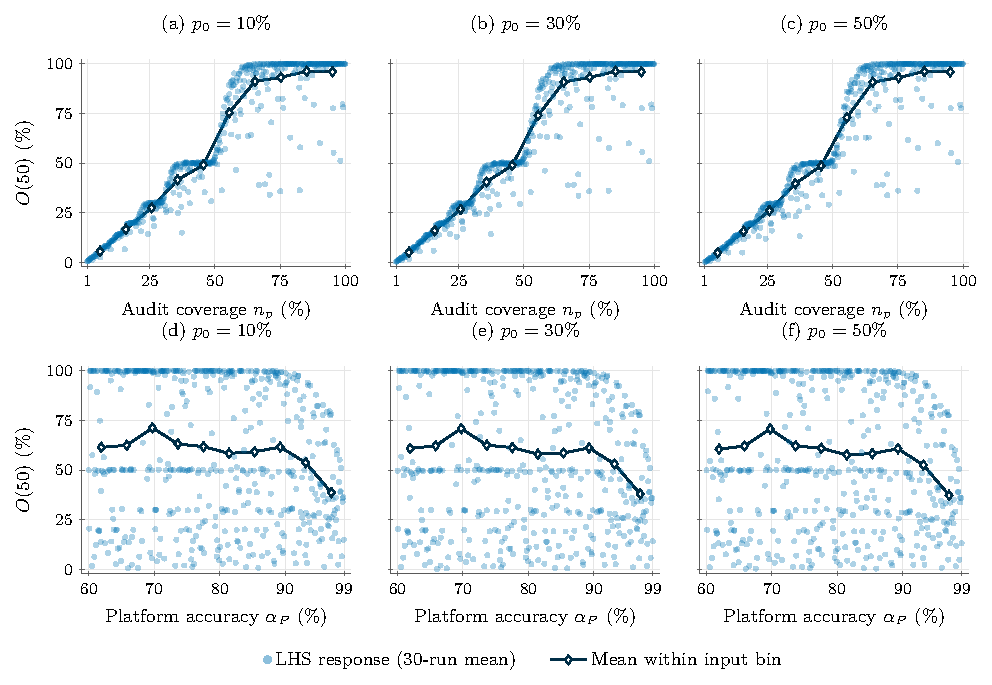
\includegraphics[width=\textwidth,height=0.78\textheight,keepaspectratio]{figures/sensitivity_response_platform_O_final.pdf}
\caption{Input--response patterns for platform governance and wrongful exposure $O(50)$. Sampling, bin summaries and interpretation follow Fig.~\ref{fig:supp-sensitivity_response_legal_E_mean}.}
\label{fig:supp-sensitivity_response_platform_O_final}
\addcontentsline{toc}{subsection}{\protect\numberline{Fig.~\thefigure}Platform input--response patterns: wrongful exposure}
\end{figure}
\clearpage
